%\documentclass[10pt]{letter}
%\usepackage[utf8]{inputenc}

%%%%%%%%%%%%%%%%%%%%%%%%%%%%%%%%%%%%%%%%%%%%%%%%%
% compile with LuaLatex
%%%%%%%%%%%%%%%%%%%%%%%%%%%%%%%%%%%%%%%%%%%%%%%%%%%%%%%
\documentclass[11pt]{report}
\usepackage{epsfig}
\usepackage{amssymb,amsmath,amsfonts}
\usepackage[activeacute,american]{babel}
%\usepackage[utf8]{inputenc}
\usepackage{subfiles}
\usepackage{cite}
\usepackage{csquotes}
\usepackage{esvect}
\usepackage[acronym,nonumberlist]{glossaries}
\renewcommand{\acronymname}{Nomenclature}

\usepackage{caption} 
\usepackage{float}
\usepackage[
    math-style=ISO,      % Upper Case Greek is in italics
    bold-style=ISO,      % Bold math is in italics
    partial=upright,     % nabla and partial upright
    nabla=upright,
  ]{unicode-math}
\topmargin 1.2cm 
\textwidth 16.1cm
\textheight 22.5cm
\oddsidemargin 0.7cm
\setcounter{tocdepth}{5}
\addtolength{\voffset}{-2.4cm}
\addtolength{\hoffset}{-0.5cm}

\usepackage{setspace}
%\doublespacing
\onehalfspacing
\usepackage{caption}
 \captionsetup[figure]{labelfont={bf},name={Figura},labelsep=period}


%%%%%%%%%%%%%%%%%%%%%%%%%%%%%%%%%
\begin{document}
\centering{ \textbf{\Large{Mec\'anica de fluidos}}}

%\centering {\Large{2$^\circ$ semestre 2020: 541209-1}}
\vspace{1cm}

\flushleft{ \large \underline{\textbf{Pr\'actica 1: Distribuci\'on de presi\'on hidrost\'atica}}}

%%%%%%%%%%%%%%%%%%%%%%%%%
\vspace{1cm}

\underline {Problema 1 (P. 3.18 , P. 3.19 Fox\footnote{footnotes working fine}):}

\vspace{0.2cm}
El estanque particionado presentado en la figura~\ref{fig:fig1} contiene agua y mercurio ($SG_{Hg}=13.56$).

a) ¿C\'ual es la presi\'on manom\'etrica del aire atrapado en la camara izquierda del estanque?

b) ¿A que presi\'on se debe bombear el aire de la c\'amara izquierda para que las alturas de los l\'iquido de ambas c\'amaras se nivelen?

c) Si la c\'amara derecha se sellara, ¿A qu\'e presi\'on se debiera bombear el aire de la camara izquierda para que las alturas de los l\'iquido de ambas c\'amaras se nivelen? (Considere que el aire de la camara derecha se comporta isot\'ermicamente)

\begin{figure}[H]
\centering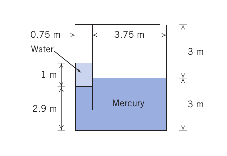
\includegraphics[width=0.5\textwidth]{Figures/3_18_3_19.eps}
\caption{\label{fig:fig1} }
\end{figure}

\footnotetext{Pritchard, Philip J. Fox and McDonald’s Introduction to Fluid Mechanics (8th ed.). John Wiley $\&$ Sons. (2011).}
%%%%%%%%%%%%%%%%%%%%%%%%%
\newpage
%%%%%%%%%%%%%%%%%%%%%%%%%

\underline {Problema 2 (P. 3.27 Fox):}

\vspace{0.2cm}

Considere el estanque presentado en la figura~\ref{fig:fig2}, que contiene mercurio ($SG_{Hg}=13.56$), agua, benceno ($SG_{benceno}=0.877$) y aire. 

a) Calcule la presi\'on manom\'etrica del aire. 
b) Si se abre un agujero en la parte superior del estanque, ¿C\'ual ser\'a el nivel de equilibrio del mercurio en el man\'ometro?.

\begin{figure}[H]
\centering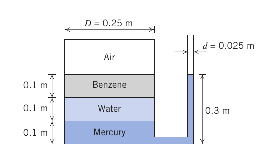
\includegraphics[width=0.5\textwidth]{Figures/3_27.eps}
\caption{\label{fig:fig2} }
\end{figure}

%%%%%%%%%%%%%%%%%%%%%%%%%
\vspace{0.5cm}
\underline {Problema 3 (P. 3.49 Fox):}
\vspace{0.2cm}

Calcule la presi\'on en los puntos A,B y C y en las cavidades de aire para el estanque representado en la figura~\ref{fig:fig3}. $SG_{MB}=1.75$

\begin{figure}[H]
\centering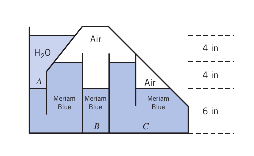
\includegraphics[width=0.5\textwidth]{Figures/3_49.eps}
\caption{\label{fig:fig3} }
\end{figure}

%%%%%%%%%%%%%%%%%%%%%%%%%
\newpage
%%%%%%%%%%%%%%%%%%%%%%%%%

\vspace{0.5cm}
\underline {Problema 4 (P. 3.68E Mott\footnote{footnotes working fine}):}
\vspace{0.2cm}

Para el man\'ometro diferencial compuesto de la figura~\ref{fig:fig4}, calcule la diferencia de presi\'on entre los puntos A y B.

\begin{figure}[H]
\centering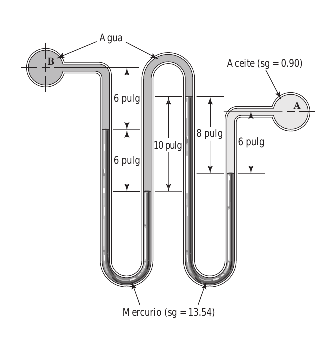
\includegraphics[width=0.5\textwidth]{Figures/3_68E.eps}
\caption{\label{fig:fig4} }
\end{figure}

\footnotetext{Mott, Robert L. Mecanica de Fluidos 6/e. Pearson educación, 2006.}

%%%%%%%%%%%%%%%%%%%%%%%%%
\newpage
%%%%%%%%%%%%%%%%%%%%%%%%%


\vspace{0.5cm}
\underline {Problema 5 (P. 2.30 Munson\footnote{footnotes working fine}):}
\vspace{0.2cm}

La figura~\ref{fig:fig5} muestra dos tuberias conectadas por un manometro. Determine la diferencia de presi\'on entre las tuberias.

\begin{figure}[H]
\centering\includegraphics[width=0.5\textwidth]{Figures/2_30M.png}
\caption{\label{fig:fig5} }
\end{figure}

\footnotetext{Munson, Bruce R., et al. "Fundamentals of Fluid Mechanics, John Wiley $\&$ Sons." Inc., USA (2006).}
%%%%%%%%%%%%%%%%%%%%%%%%%


\vspace{0.5cm}
\underline {Problema 6 (P. 2.45 Munson):}
\vspace{0.2cm}

Determine la nueva lectura en el manometro presentado en la figura~\ref{fig:fig6} para el caso en que la presi\'on en la tuberia A disminuye en $10$ kPa

\begin{figure}[H]
\centering\includegraphics[width=0.5\textwidth]{Figures/2_45M.png}
\caption{\label{fig:fig6} }
\end{figure}

%%%%%%%%%%%%%%%%%%%%%%%%%
\newpage
%%%%%%%%%%%%%%%%%%%%%%%%%

\vspace{0.5cm}
\underline {Problema 7 (P. 2.53 Munson):}
\vspace{0.2cm}

Un pist\'on de diametro $6$\,in se conecta a un cilindro, el cual a su vez est\'a conectado a un manometro de tubo inclinado de diametro $1/2$\,in. El fluido al interior del cilindro y man\'ometro corresponde a un aceite con $\gamma=59$\,lb/ft$^3$. Al colocar un objecto de peso $W$ sobre el piston, el nivel en el man\'ometro aumenta del punto $1$ al punto $2$. Calcule el peso $W$ del objecto. Suponga que el cambio de posici\'on en el pist\'on es despreciable.

\begin{figure}[H]
\centering\includegraphics[width=0.5\textwidth]{Figures/2_53M.png}
\caption{\label{fig:fig6} }
\end{figure}
%%%%%%%%%%%%%%%%%%%%%%%%%
\end{document}
